% chapters/cap3_marcoteorico/cap3.tex

\chapter{Marco Teórico y Estado del Arte}
\label{ch:marco_teorico}

Para comprender la propuesta de este trabajo, es necesario establecer las bases físicas y computacionales que rigen el problema que se quiere afrontar. Este capítulo da una breve descripción desde los fundamentos clásicos de la dinámica de fluidos computacional (CFD), haremos más hincapié en la formulación SPH ya que es el foco principal, veremos el significado físico de la ecuación de advección y bases para comprender el apoyo de las caminatas cuánticas de tiempo continuo (CTQW).

\section{Simulación de fluidos: Malla vs. SPH}

La mecánica de fluidos computacional tiene dos formulaciones con enfoques diferentes, el primero es el enfoque euleriano, de malla el cual ilustra el fluido desde fuera y el enfoque lagrangiano, de partículas, el cual intenta describir el fluido por la interacción de las partículas. Conocer sus límites resulta imperativo, pues sus cuellos de botella clásicos alimentan la búsqueda de aceleración cuántica.

\subsection*{Métodos basados en malla (eulerianos)}
En los métodos de malla —FVM, FEM, FDM— el dominio se escinde en celdas fijas a través de las cuales las propiedades del fluido migran en el tiempo.

\begin{itemize}
    \item \textbf{Fortalezas:} Constituyen el estándar de la industria aeronáutica y automotriz. Gozan de sólidos fundamentos matemáticos, conservación estricta de flujos y precisión geométrica insuperable para configuraciones estables.
    \item \textbf{Fragilidades:} Ante cambios topológicos —superficies libres, deformaciones extremas o interacción fluido-estructura— exigen remallado dinámico, lo que encarece el cálculo hasta volverlo inviable y propaga inestabilidades numéricas.
\end{itemize}

\subsection*{Métodos de partículas: SPH (lagrangianos)}
El \emph{Smoothed Particle Hydrodynamics} renuncia a la malla. El fluido se atomiza en partículas autónomas que portan masa y presión, y el sistema evoluciona por interacciones vecinales.

\begin{itemize}
    \item \textbf{Fortalezas:} Captura con naturalidad salpicaduras, roturas e impactos violentos. Al suprimir la fase de mallado —que en proyectos industriales consume semanas—, el tiempo de preparación se reduce drásticamente.
    \item \textbf{Fragilidades:} Las condiciones de contorno resultan matemáticamente esquivas, y la resolución fina exige masas de partículas que empalidecen la parsimonia de los métodos de malla.
\end{itemize}

\begin{figure}[htbp]
    \centering
    \begin{minipage}[t]{0.48\textwidth}
        \centering
        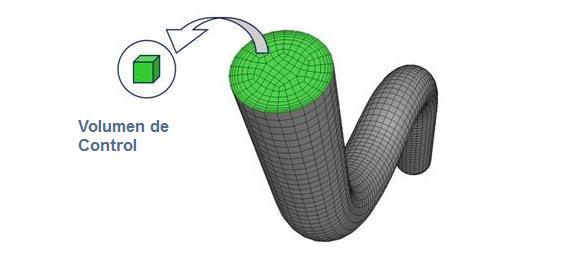
\includegraphics[width=\textwidth]{chapters/cap3_macro/img/malla.jpg}
        \captionof{figure}{Discretización de volumen de control mediante enfoque Euleriano \cite{esss_cfd}.}
        \label{fig:malla}
    \end{minipage}
    \hfill
    \begin{minipage}[t]{0.48\textwidth}
        \centering
        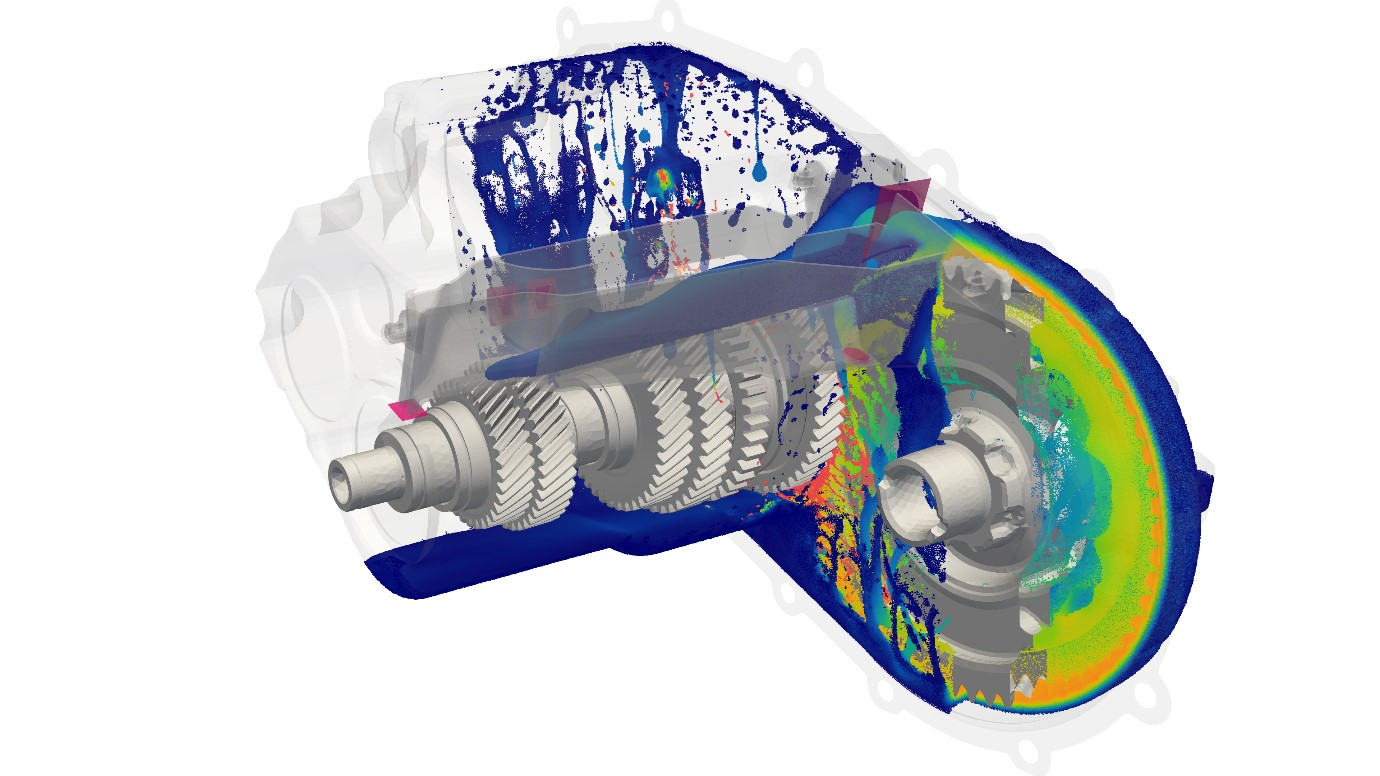
\includegraphics[width=\textwidth]{chapters/cap3_macro/img/sph.jpg}
        \captionof{figure}{Simulación altamente dinámica mediante SPH, sin necesidad de remallado \cite{nextflow_sph_2020}.}
        \label{fig:sph}
    \end{minipage}
\end{figure}


\subsection{Complejidad en métodos de malla}

En la CFD clásica por malla, el cuello de botella es de carácter \textbf{global}: surge al linealizar y resolver los grandes sistemas algebraicos (matrices dispersas) derivados de las ecuaciones de Navier-Stokes. 

Para un dominio 3D discreto con $N$ nodos por dimensión, el número de grados de libertad es $n \sim cN^3$ (donde $c$ es el número de variables por nodo). Un tratamiento directo denso exigiría tiempos inasumibles de $O(n^3) = O(N^9)$. En la práctica, códigos industriales como FUN3D (NASA) o CODA (DLR) emplean métodos iterativos de Krylov (como GMRES) explotando la matriz dispersa. Según el estudio de Wood et al. \cite{Wood2020SLAT} y Wagner \cite{Wagner2021CODASpliss}, el coste temporal por paso de simulación se aproxima a:
\[
C_{\text{Malla}} \sim O(k \cdot N^3)
\]
donde $k$ es el número de iteraciones del solver (dependiente del precondicionador y la física del flujo). Aunque esta complejidad no es matemáticamente exponencial, las exigentes constantes de cálculo, la sincronización de memoria y la resolución de turbulencia hacen que este coste siga siendo un reto masivo de cara a la agenda \textit{CFD Vision 2030} \cite{Slotnick2014CFDV2030}. La resolución de este sistema lineal llega a consumir entre el 50\% y el 90\% del tiempo de simulación \cite{Wood2020SLAT}.


\subsection{Complejidad en SPH}

Para entender de una manera más intuitiva la complejidad del método de SPH se puede consultar la siguiente sección \ref{sec:sph}, en donde se introduce la formulación SPH. Principalmente la complejidad radica en dos etapas, la búsqueda de partículas vecinas con las que una sola interactúa y su posterior procesamiento.

Para un sistema con $M$ partículas, el método más rudimentario consiste en evaluar la interacción directa de cada partícula con todas las demás (\textit{All-pair search}), para comprobar si una determinada partícula está dentro del radio de interacción de otra. Como se describe en \cite{liu2003sph}, esto implica un coste computacional cuadrático $O(M^2)$, inviable para aplicaciones reales. Para evitarlo, se aprovecha el radio de soporte compacto del kernel (denotado como $h$) mediante algoritmos de estructuración espacial, reduciendo drásticamente las interacciones computadas:

\begin{itemize}
    \item \textbf{Búsqueda por Árboles (ej. Octrees):} Estructuran el dominio de forma jerárquica logrando un coste $O(M \log M)$. Son necesarios cuando las partículas poseen longitudes de suavizado ($h$) variables y adaptativas.
    \item \textbf{Listas enlazadas (\textit{Linked-lists}):} En lugar de comparar cada partícula una con otra, se divide el espacio en una cuadrícula y se mide la distancia de una partícula con otra solo si están en la misma celda o si están en celdas vecinas. Esto puede llegar a alcanzar una complejidad teórica óptima de $O(M)$. Pero no es tan eficiente con longitudes de suavizado ($h$) variables.
\end{itemize}

A pesar de que el algoritmo de búsqueda puede optimizarse a niveles de $O(M)$, SPH exige un esfuerzo computacional masivo. La limitación de SPH como vemos no es la acotación de listas de interacciones, sino tres factores físicos y de hardware:

\begin{enumerate}
    \item \textbf{Carga aritmética local:} En SPH 3D, una sola partícula puede interactuar con algunas partículas hasta cientos de vecinos. Para cada par, el procesador debe calcular su respectiva distancia, interpolar el polinomio del kernel $W(r,h)$ y evaluar sus gradientes espaciales para las fuerzas físicas \cite{liu2003sph}. Para simular $M$ partículas, esto significa realizar cientos de millones de operaciones matemáticas por cada instante de tiempo.
    
    \item \textbf{Memoria (\textit{Cache Misses}):} A diferencia de una malla estática donde los datos son contiguos, la naturaleza móvil de las partículas SPH provoca que vecinos físicamente cercanos en el espacio tridimensional estén almacenados en posiciones aleatorias de la memoria RAM. Este acceso desordenado destruye la coherencia de caché. Las CPUs y GPUs desperdician la mayor parte del tiempo esperando a que los datos lleguen de la memoria principal en lugar de realizar cálculos \cite{Staubach2010SPHSystemSimulation}.
    
    \item \textbf{Restricción temporal (Condición CFL):} Para garantizar la estabilidad de la integración numérica, el paso de tiempo $\Delta t$ está limitado por la condición de Courant-Friedrichs-Lewy (CFL). El avance debe ser minúsculo (del orden de microsegundos) para capturar la acústica y el movimiento sin que las partículas crucen a otros dominios repentinamente \cite{Mocz2020SPH}. Esto obliga a calcular repetitivamente toda la búsqueda espacial y la aritmética para las partículas decenas de miles de veces para simular un solo segundo de realidad.
\end{enumerate}

Con esta información podemos ver que, mientras la malla tradicional es limitada en resoluciones algebraicas globales $O(N^3)$ y en cambio el formalismo SPH es limitado localmente. Su barrera no es la complejidad matemática de la búsqueda, sino la inmensa densidad de cálculo combinatorio, el acceso errático a la memoria clásica y la fragmentación temporal. Estos límites clásicos son los que justifican directamente la exploración de otros métodos.


\section{La ecuación de advección unidimensional}
\label{sec:adcevtion}

Es importante para el lector entender el fenómeno físico que este trabajo busca simular. En mecánica de fluidos, la advección se define como el transporte de una cantidad escalar (como la masa, la temperatura o un contaminante) por el movimiento macroscópico o \emph{bulk motion} de un campo de velocidades \cite{leveque2002finite}.

La ecuación de advección es una ecuación diferencial parcial hiperbólica de primer orden que gobierna este transporte. En su forma más fundamental y asumiendo un flujo incompresible en una dimensión ($1D$), la ecuación se expresa como:
\begin{equation}
    \frac{\partial f}{\partial t} + c \frac{\partial f}{\partial x} = 0
    \label{ec: advection}
\end{equation}

donde $f(x,t)$ es la cantidad o propiedad escalar que está siendo advectada, $t$ es el tiempo, $x$ es la coordenada espacial y $c$ representa el campo de velocidad constante del fluido.

El significado físico de esta ecuación radica en la conservación de la propiedad a lo largo del flujo; establece que la tasa de cambio local de $f$ en un punto fijo depende directamente del gradiente espacial de la propiedad y de la velocidad con la que el fluido la arrastra. En el contexto de este trabajo, la resolución de la ecuación de advección 1D es de vital importancia, ya que constituye el problema de referencia más simple para aislar y validar el comportamiento de transporte de nuestro algoritmo cuántico. Con dos nodos fijos, \eqref{eq:sph_advection_discrete} no realiza ese transporte a lo largo de características, ya que se una produce reljación hacia la media.


\section{Formulación SPH y discretización de la advección}
\label{sec:sph}

La base matemática del \textit{Smoothed Particle Hydrodynamics} (SPH) se fundamenta en la teoría de la interpolación a través de la propiedad de filtrado de la función delta de Dirac. Para una función continua arbitraria $f(x)$, esta propiedad establece que el valor de la función en un punto se puede obtener como una integral definida en el dominio $\Omega$:
\begin{equation}
    f(x) = \int_{\Omega} f(y) \delta(x - y) dy
    \label{eq:dirac_property}
\end{equation}
Sin embargo, en el método SPH no se puede trabajar con la singularidad matemática de la delta de Dirac. En su lugar, esta distribución se reemplaza por una función de aproximación conocida como \textit{kernel} de suavizado $W(r, h)$. Este kernel aproxima la función continua mediante:
\begin{equation}
    f(x) \approx \int_{\Omega} f(y) W(x - y, h) dy
    \label{eq:kernel_approximation}
\end{equation}
donde $h$ es la longitud de suavizado (\textit{smoothing length}) que define el radio de soporte compacto del kernel, y $r = |x - y|$ es la distancia entre el punto de interés y sus vecinos. 

El \textit{kernel} es, en esencia, la función geométrica que describe la intensidad de la interacción entre una partícula y su entorno local (véase la figura \ref{fig:kernel_sph}). Al definir el kernel de una forma geométrica conocida, con SPH se logra calcular las derivadas de campos continuos de forma analítica trasladando el operador diferencial a ese kernel, evitando la necesidad de mallas.

\begin{figure}[htbp]
    \centering
    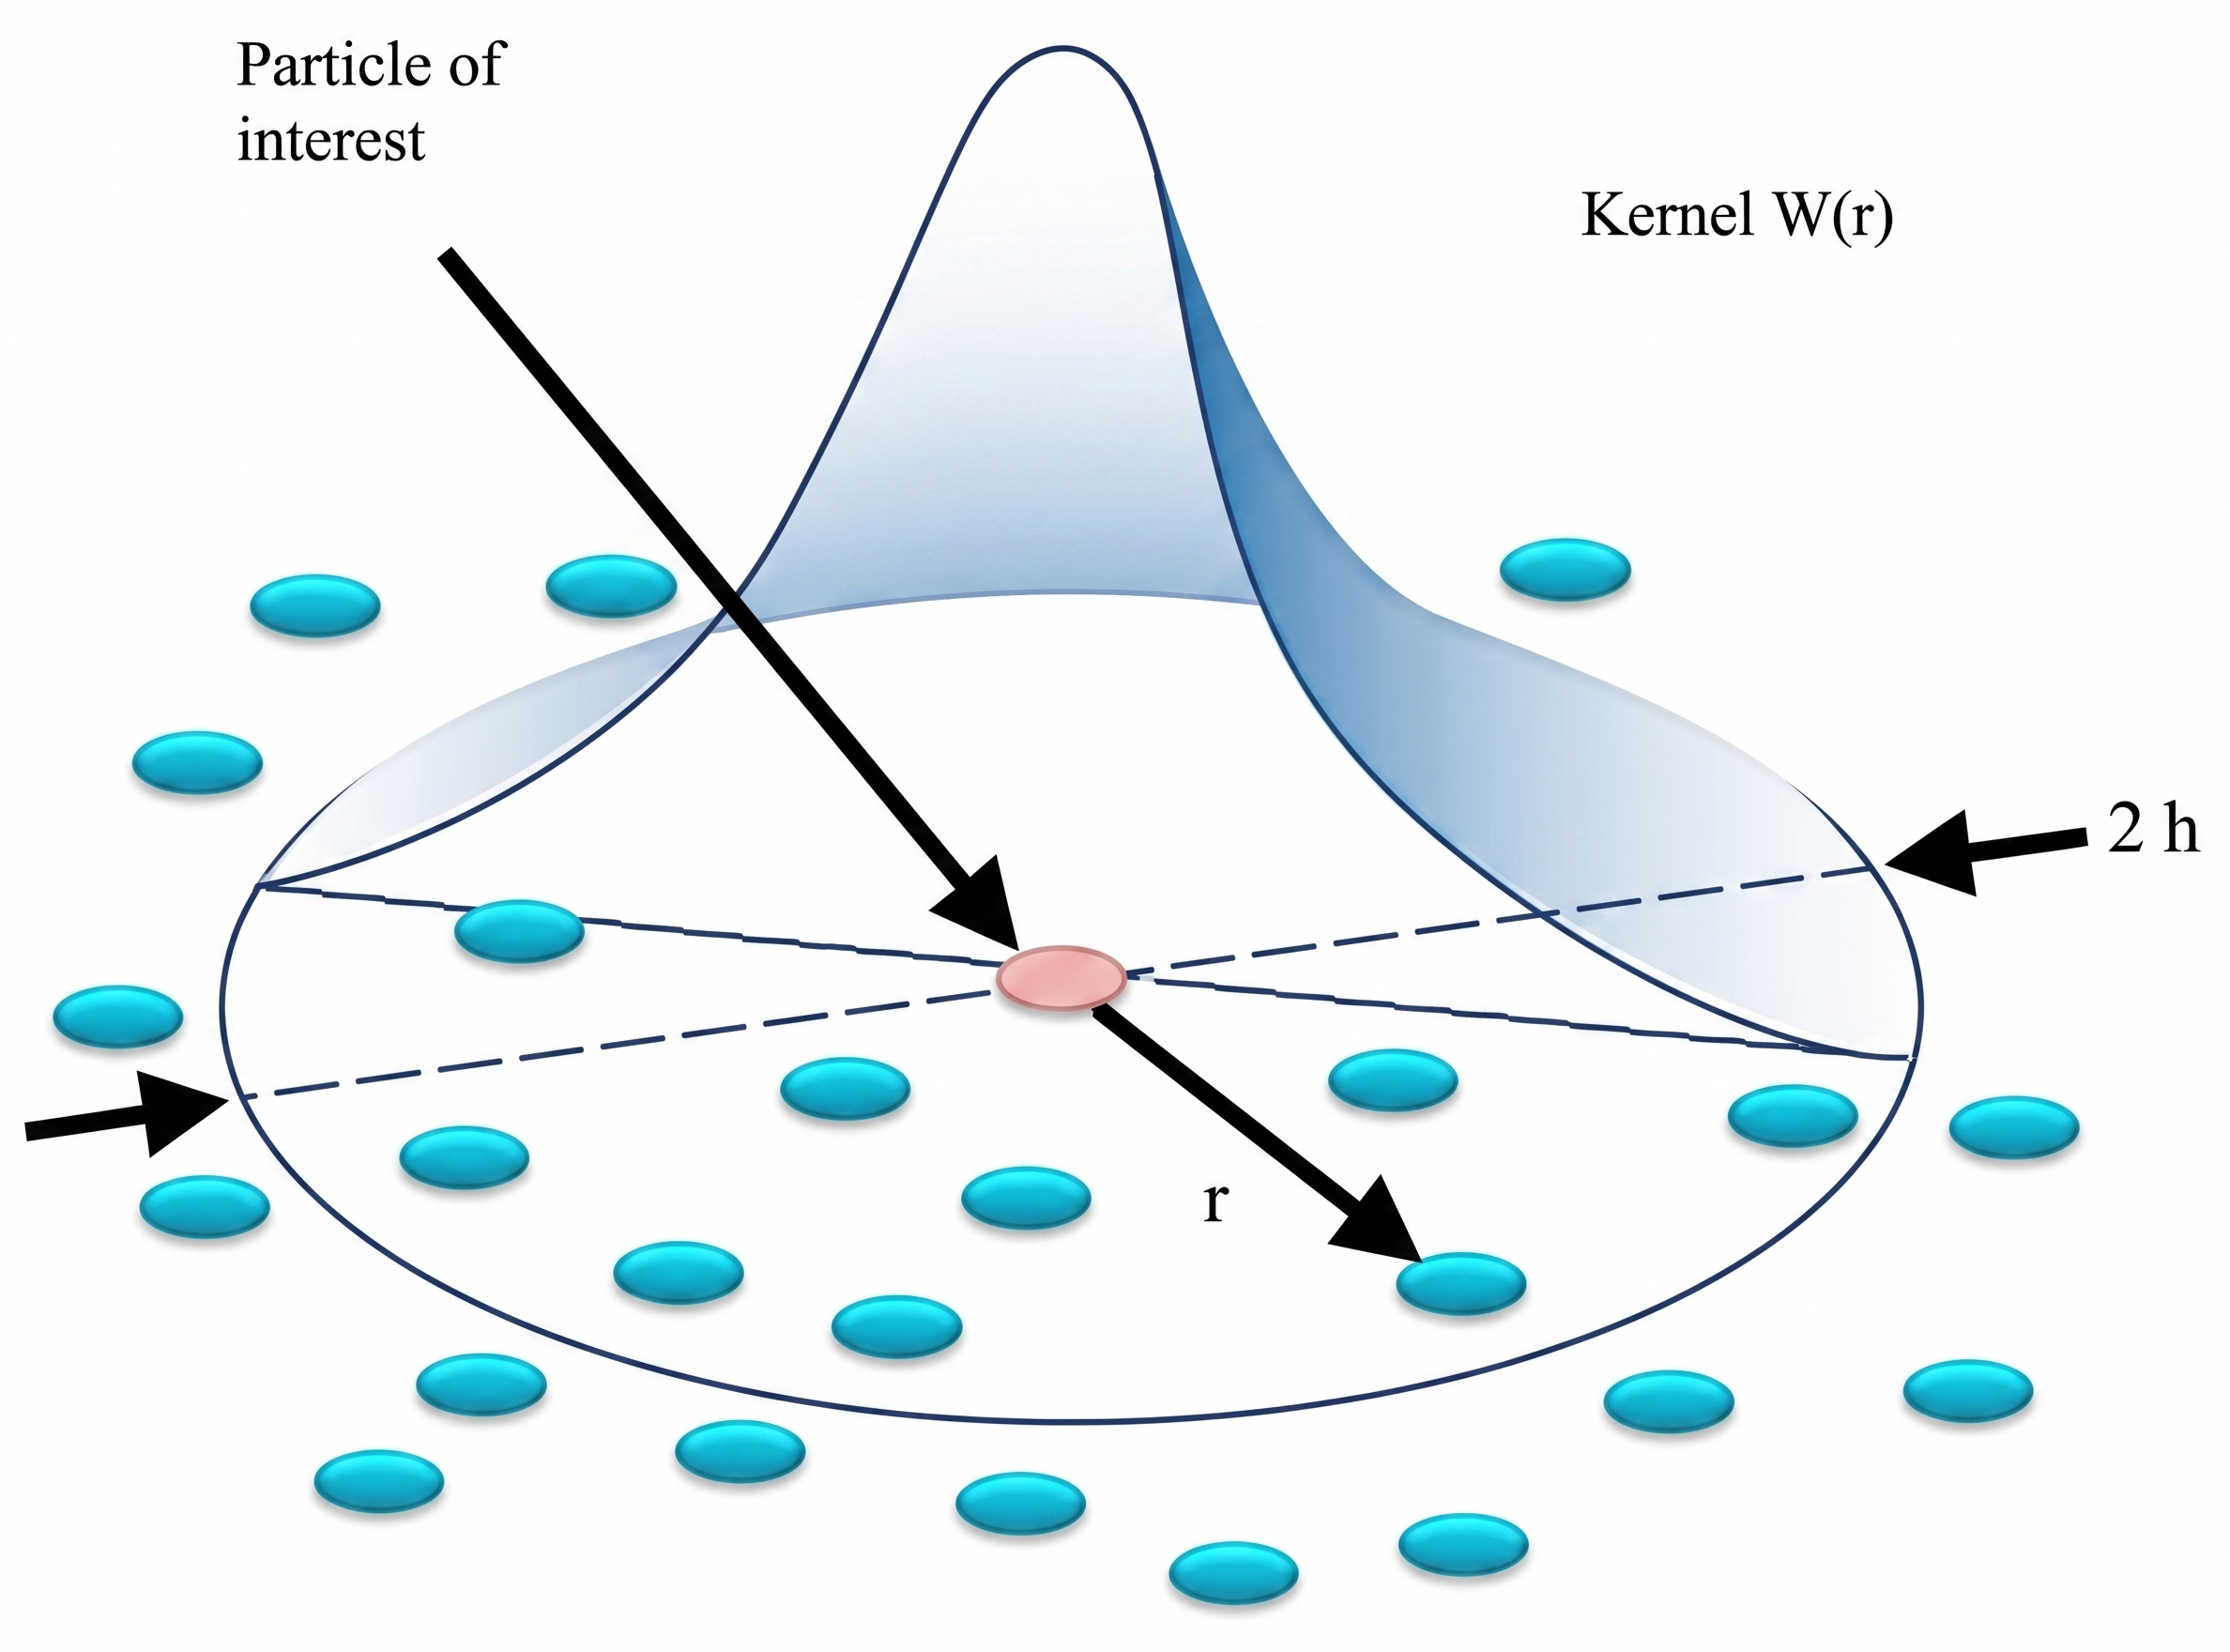
\includegraphics[width=0.6\textwidth]{chapters/cap3_macro/img/kernelsph.png}
    \caption{Representación visual de la función de kernel $W(r, h)$ sobre un sistema de partículas. El parámetro $h$ define el límite del soporte compacto, fuera del cual las interacciones entre partículas se asumen nulas.}
    \label{fig:kernel_sph}
\end{figure}

Al pasar de una integral continua a una sumatoria sobre partículas discretas, el fluido deja de tratarse como un volumen continuo y pasa a representarse como una nube de puntos interactuantes (Figura \ref{fig:sph_difu}). El resultado es un sistema mecánico discreto donde las partículas evolucionan en función de sus distancias mutuas, lo que hace al SPH inherentemente compatible con la formulación lagrangiana y hamiltoniana de la física.

\begin{figure}[htbp]
    \centering
    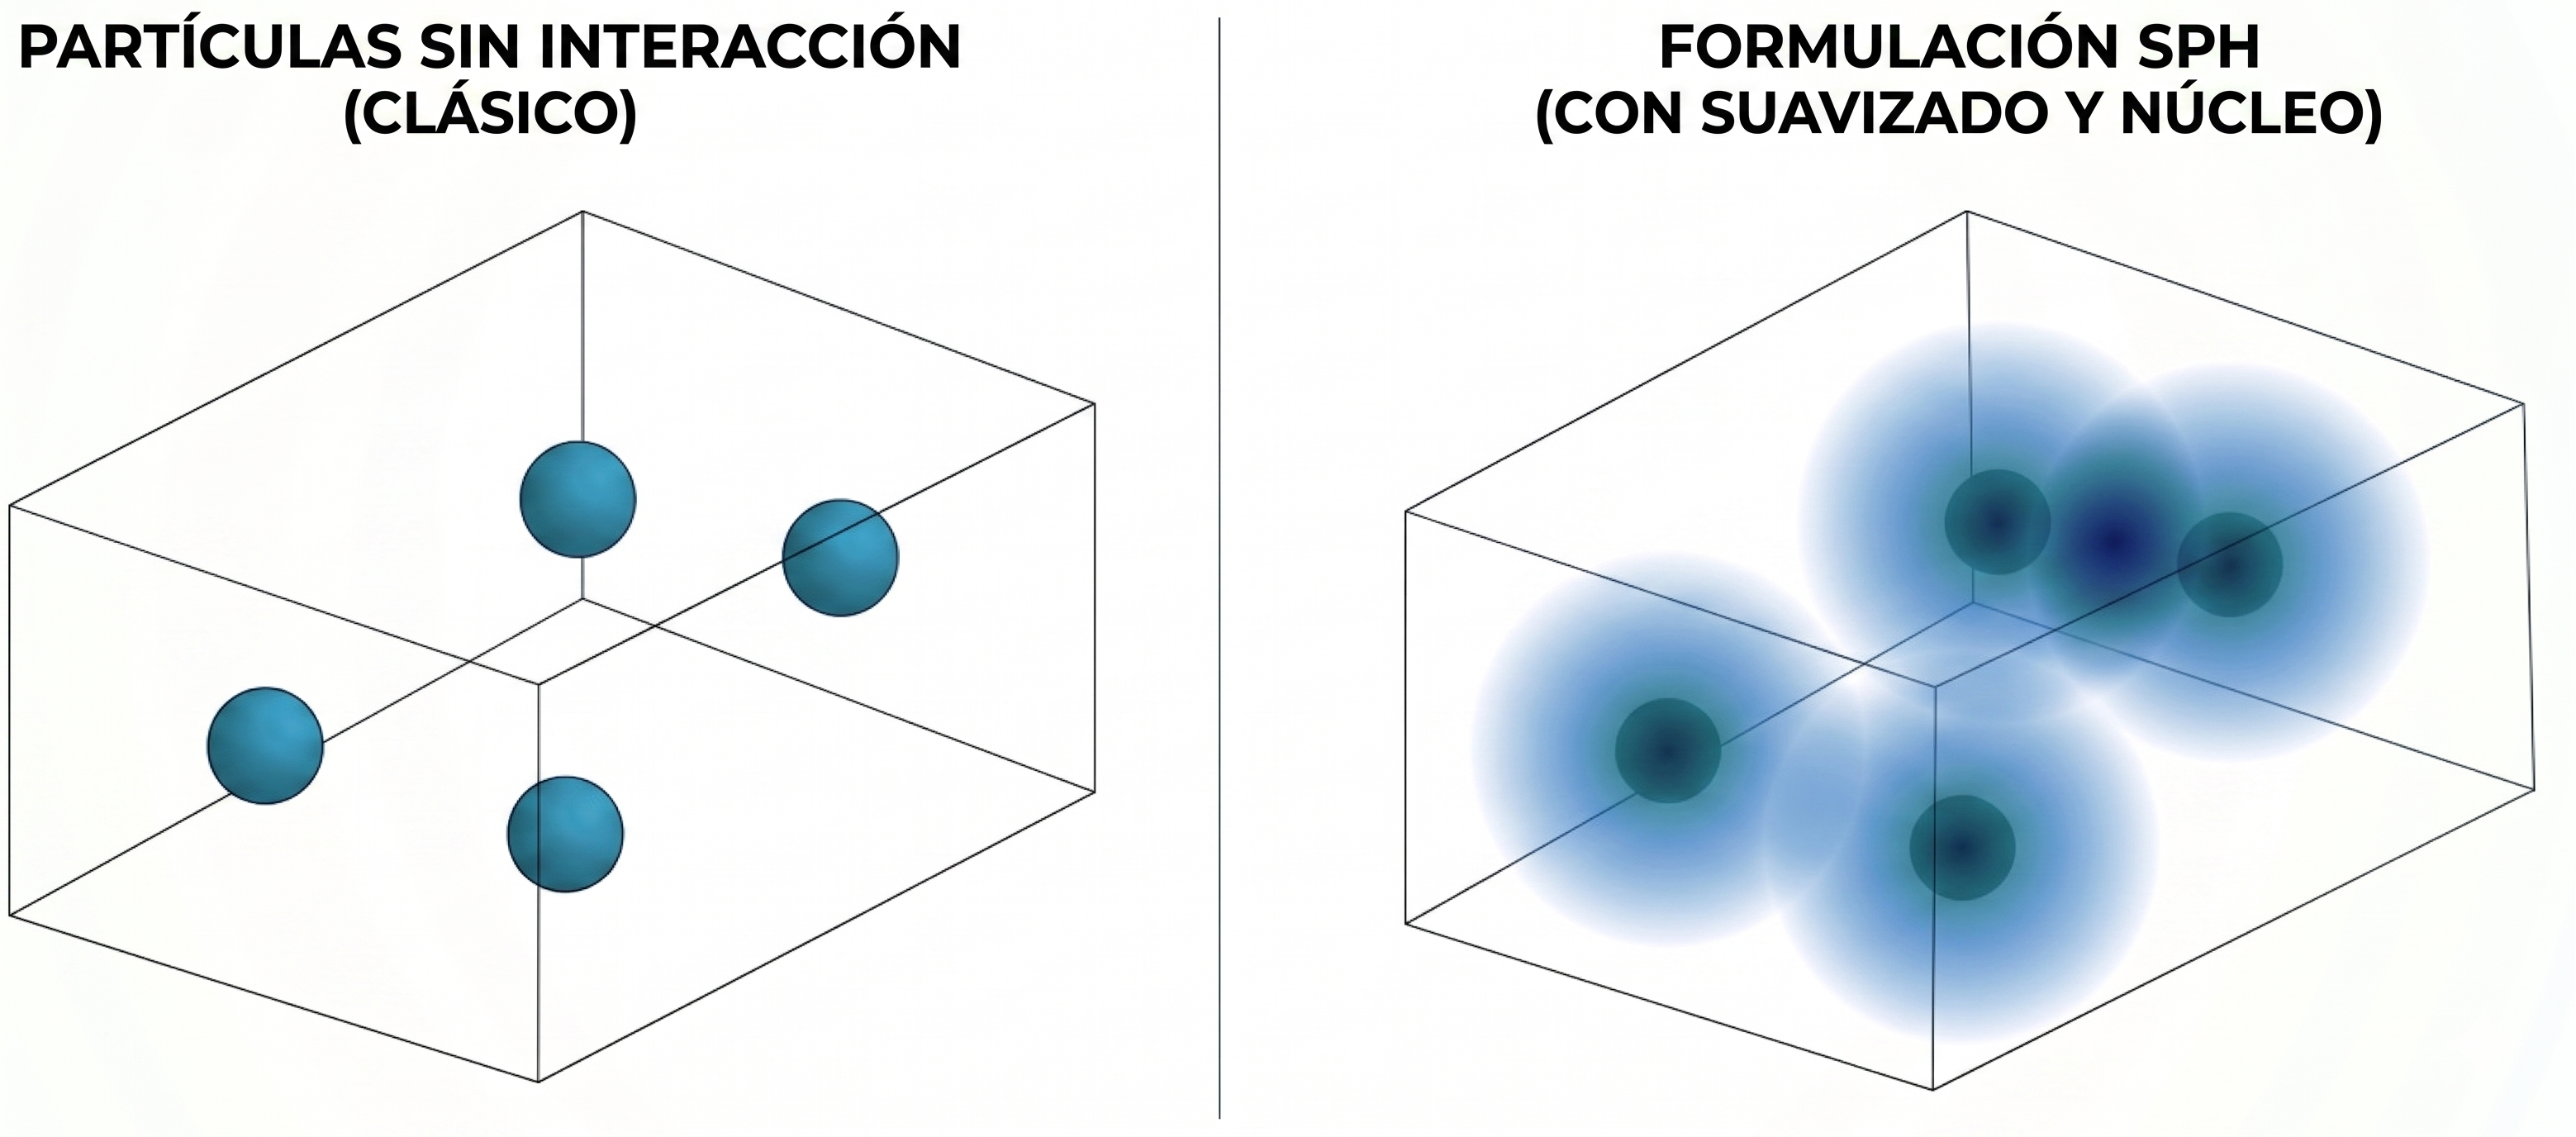
\includegraphics[width=0.8\textwidth]{chapters/cap3_macro/img/sphdifu1.png}
    \caption{Visualización conceptual de la interacción en SPH. Izquierda: partículas discretas separadas sin aparente conexión. Derecha: Difuminación de la partícula que permite solapar sus ``estelas'' o zonas de influencia, generando interacciones (definidas por el kernel) a pesar de la distancia física.}
    \label{fig:sph_difu}
\end{figure}

\subsection{Discretización de la ecuación de advección 1D}

Para comprender la ejecución computacional de este sistema discreto, tomaremos como modelo base la ecuación de advección lineal en 1D (\ref{ec: advection}). Como se definió previamente en la sección \ref{sec:adcevtion}, esta ecuación describe el transporte de una cantidad escalar a una velocidad de advección $c$, esta cantidad la llamaremos $u(x,t)$: 
\begin{equation}
    \frac{\partial u(x,t)}{\partial t} + c \frac{\partial u(x,t)}{\partial x} = 0
    \label{eq:advection_continuous}
\end{equation}

El propósito de discretizar esta ecuación es transformar la variable continua dependiente del espacio $u(x,t)$ en un conjunto finito de variables $u_j(t)$, correspondientes a cada partícula $j$ simulada en el ordenador \cite{auyeung2025}.

Aplicando la aproximación de partículas SPH al gradiente espacial de la cantidad $u$, se transita de la forma continua a una sumatoria de interacciones ponderadas por la derivada del kernel $\nabla_j W_{jk}$. Sustituyendo en la ecuación de advección diferencial y despejando para el siguiente instante temporal $t + \Delta t$ usando un esquema de Euler explícito, se obtiene la expresión completamente discretizada \cite{auyeung2025}:
\begin{equation}
    u_j(t_0 + \Delta t) = u_j(t_0) - c \Delta t \sum_{k \in \mathcal{N}_j} \left( u_k(t_0) - u_j(t_0) \right) \nabla_j W_{jk}
    \label{eq:sph_advection_discrete}
\end{equation}
donde:
\begin{itemize}
    \item $u_j(t_0)$ es el valor de la advección para la partícula de interés $j$ en el tiempo inicial $t$.
    \item $c$ es la velocidad constante de advección.
    \item $\Delta t$ es el paso de integración temporal.
    \item $\mathcal{N}_j$ representa el conjunto de partículas vecinas $k$ contenidas dentro del radio de influencia delimitado por $h$.
    \item $\nabla_j W_{jk}$ es el gradiente de la función de suavizado de la partícula $j$ con respecto a la partícula vecina $k$.
\end{itemize}

Esta formulación (ecuación \ref{eq:sph_advection_discrete}) encapsula la esencia computacional del método SPH ya que, el estado futuro de la partícula $j$ no depende de una cuadrícula estática, sino de la suma de las interacciones con sus partículas vecinas $k$, regidas por la geometría. En el caso de dos partículas fijas, ambas permanecen dentro del soporte del kernel y la ecuación~\eqref{eq:sph_advection_discrete} produce una relajación hacia la media $u=1/2$, que es precisamente el comportamiento de la referencia clásica del capítulo~\ref{cap:resultados}.



\section{Continuous-Time Quantum Walks (CTQW)}
Para llegar a una solución del advectivo planteado en la ecuación (\ref{eq:sph_advection_discrete}), en este trabajo se plantean las caminatas cuánticas. Las caminatas cuánticas en tiempo continuo (CTQW) son la contraparte cuántica de las caminatas aleatorias clásicas (procesos de Markov), formuladas originalmente para la exploración de grafos y espacios de estados discretos en computación \cite{VenegasAndraca2012}.

En un CTQW, el ``caminante'' no se mueve mediante decisiones probabilísticas paso a paso. En cambio, su amplitud de probabilidad evoluciona de manera continua a lo largo del tiempo bajo un escenario planteado por el hamiltoniano $H$ y gobernado por la ecuación de Schrödinger:
\begin{equation}
    i\hbar \frac{d}{dt} |\psi(t)\rangle = H |\psi(t)\rangle
\end{equation}

En la teoría de grafos cuánticos, el hamiltoniano $H$ que rige esta evolución se define directamente a través de la matriz de adyacencia $A$ del grafo (o su Laplaciano $L$). De este modo, la evolución unitaria temporal del estado cuántico está dada por el operador $U(t) = e^{-iHt}$. Esta característica hace a los CTQW una herramienta interesante para la simulación física, ya que, la dinámica del sistema modela fielmente las tasas de transición directa entre los nodos \cite{VenegasAndraca2012}.
